\documentclass[]{article}
\usepackage[margin=1in]{geometry}
\usepackage[english]{babel}
\usepackage{lastpage}
\usepackage{fancyhdr}
\usepackage[bottom]{footmisc}
\usepackage{titlesec}
\usepackage{caption}
\usepackage{graphicx}
\usepackage{placeins}
\usepackage{amsmath}
\usepackage{float}
\usepackage[hidelinks, final]{hyperref}

\title{
    To what extent will quantum computing systems replace high-performance computing (HPC) systems regarding computational biology? \\
    \vspace{1cm}
    \large{Centre Name: NCLT New College Pontefract}\\
    \large{Centre Number: 38185}\\
    \large{Qualification Code: 7993}\\
}

%  set up header and footer
\pagestyle{fancy}
\fancyhf{}
\lhead{Henry Philip Groves - L0034335\newline Quantum Computing and Biological Modelling}
\rhead{New College Pontefract - Centre Number: 38185}
\lfoot{Qualification Code 7993}
\cfoot{\thepage\ of \pageref{LastPage}}

% edit line spacing
\renewcommand{\baselinestretch}{1.35} 

\hypersetup{
    colorlinks=false,
    pdftitle={..},
    pdfauthor={Henry Philip Groves - L0034335}
}

\graphicspath{ {./images/} }

\setcounter{tocdepth}{5}
\setcounter{secnumdepth}{5}
% editing paragraph heading formatting
\titleformat{\paragraph}[hang]{\small\bfseries}{\theparagraph.}{0.4em}{}

% editing subparagraph heading formatting
\titleformat{\subparagraph}[hang]{\small\bfseries}{\thesubparagraph.}{0.4em}{}
\titlespacing*{\subparagraph}{0em}{3.25ex plus 1ex minus .2ex}{1em}

\titleformat{\section}[display]{\centering\bfseries\huge}{}{}{}


\author{Henry Philip Groves - L0034335}


\date{February 2023}

\begin{document}

\maketitle

\newpage
\pdfbookmark{\contentsname}{toc}
\tableofcontents


\newpage
\FloatBarrier
\phantomsection
\addcontentsline{toc}{section}{Introduction}
\section*{Introduction}

Quantum Computing is a methodology of computation that harnesses quantum mechanics. The concept of simulating quantum-mechanical systems using a computational device has been around for over 40 years, \cite{feynman_1982} however, it is only recently that the technology has matured enough to show its potentially disruptive qualities. Their inherent parallel nature and exponential scaling with size means that it can solve problems outside the problem space of classical computers. The four main areas it has an advantage  are: combinatorial optimisation, linear algebra, differential equations and factorisation. Differential equations are particularly useful in nearly all aspects of computer modelling. Specifically, I will be looking at their usage in the modelling of biological molecules.


\phantomsection
\addcontentsline{toc}{subsection}{Fundamentals}
\subsection*{Fundamentals}

\phantomsection
\addcontentsline{toc}{subsubsection}{Classical Computing}
\subsubsection*{Classical Computing}

Classical Computing, or Binary Computing, is what underpins all of our current computer systems. Information in these systems are represented in units called bits \cite{bit_definition}. Physically, these units are represented by transistors, which are small electrical switches, that can store a charge. When the transistor is ``full'' of charge, that represents that bit being ``on'', or in the Binary number system, 1. When the transistor is ``empty'', that represents the bit being off, or a 0. These switches can be combined with other components to create logic gates \cite{logic_gate_definition}, and then our modern computer systems are built from these basic gates.

\phantomsection
\addcontentsline{toc}{subsubsection}{Quantum Computing}
\subsubsection*{Quantum Computing}
Similar to Classical Systems, Quantum Computers are based on ``quantum bits'', or Qubits. However, unlike classical bits, qubits are two-dimensional vectors. Graphically, this can be represented using a Bloch sphere. See \autoref{fig:bloch_sphere}.

\begin{figure}[H]
	\centering
	\[ 0 \rightarrow | 0 \rangle = \begin{bmatrix} 1 \\ 0 \end{bmatrix} \]
	\vspace{-0.2cm}
	\[ 1 \rightarrow | 1 \rangle = \begin{bmatrix} 0 \\ 1 \end{bmatrix} \]
	\caption*{Mapping of Classical Bits to Dirac notation \cite{dirac_notation} and column vectors}
\end{figure}

\begin{figure}[H]
	\centering
	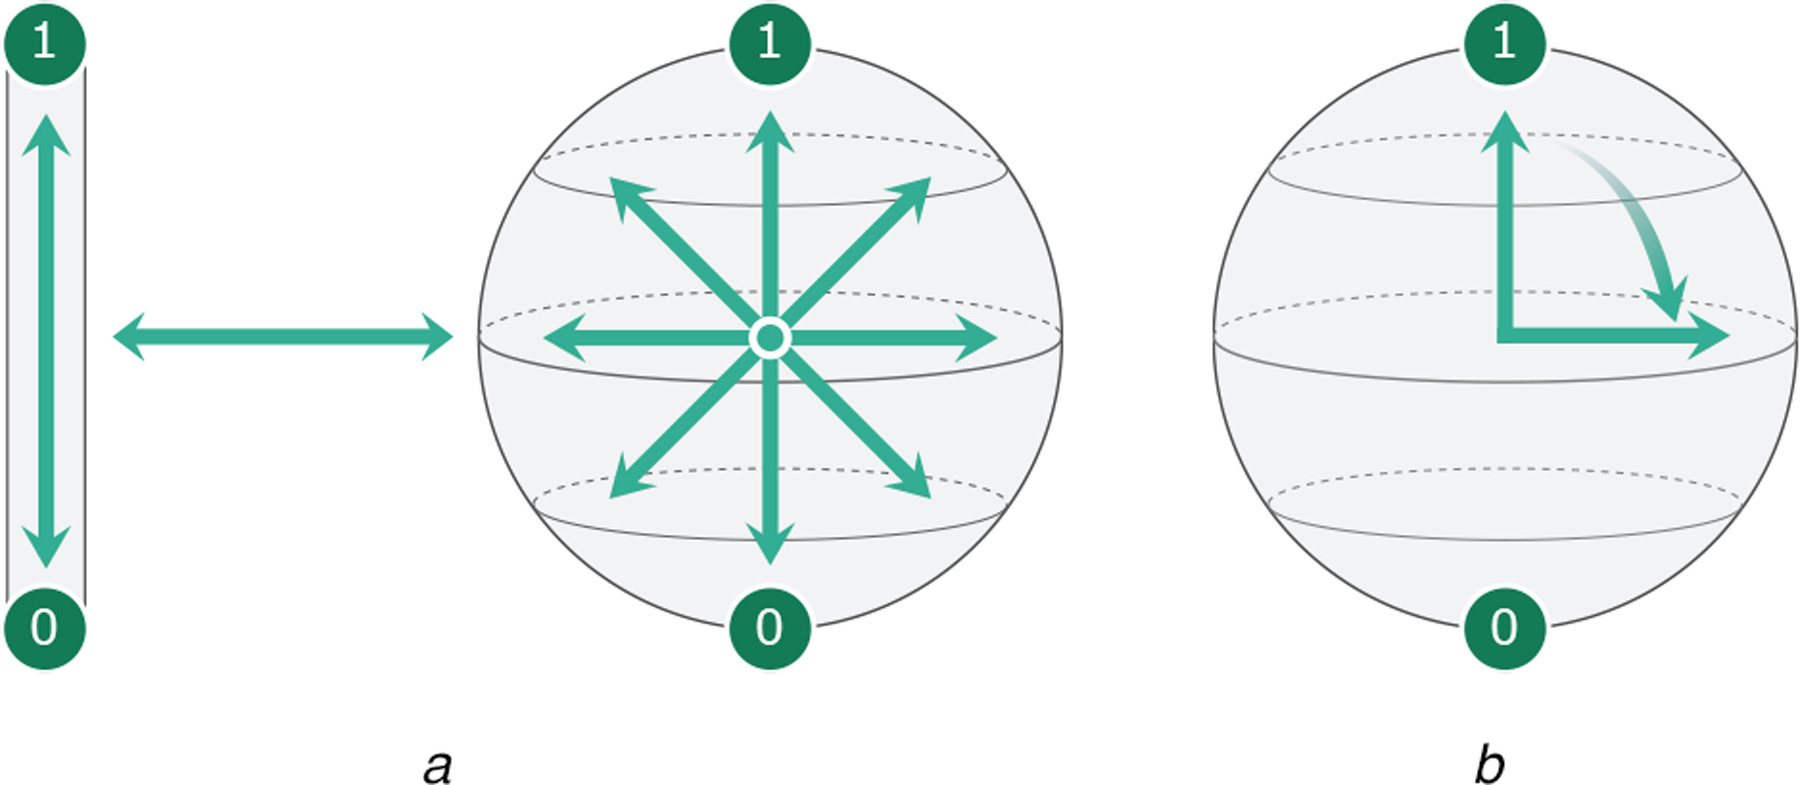
\includegraphics[width=0.65\textwidth]{blochsphere.jpg}
	\caption{a. Graphical Representation of a Qubit b. Hadamard Gate \cite{present_landscape_q}}
	\label{fig:bloch_sphere}
\end{figure}

The qubits $|0\rangle$ and $|1\rangle $ are referred to as $\{|0\rangle, |1\rangle\}$, the computational basis. This is the two basis states composed by any of the two distinct quantum states that the selected implementation of qubit can physically be in. For example, if we were using the spin \cite{quantum_spin} of a proton, where spin-up is our $|0\rangle$ state, and spin-down is our $|1\rangle$ state, then the computational basis of this qubit would be $\{|\uparrow\rangle, |\downarrow\rangle\}$.

Where qubits diverge from their classical analog is that qubit states are not discrete, meaning that they are not 0 OR 1. Instead, they exist in a superposition \cite{superposition} of both $|0\rangle$ and $|1\rangle$ states. When the value of the qubit is measured, it ``collapses'' to either $|0\rangle$ or $|1\rangle$. Whilst it cannot be predicted which state the qubit will collapse, the probability of whether a qubit will collapse to a particular state can be determined.

Analogous to classical computing, quantum computers also have quantum gates, which transform the input qubit, and large sequences of these gates can be used to perform more complex operations. More specifically, a quantum gate specifies how the computation basis (for example, $\{|0\rangle, |1\rangle\}$) is transformed by the operation of a quantum gate. The most common quantum gates are the \texttt {NOT(X)}, Hadamard gate and \texttt {CNOT(CX)}. The \texttt {NOT} gate transforms $|0\rangle$ to $|1\rangle$, and vice versa. The Hadamard gate creates an equal superposition state, therefore meaning that the input qubit has an equal chance to collapse to $|0\rangle$ or $|1\rangle$. Graphically, we can represent this by a rotation of $\pi^c$ in the Bloch Sphere \cite{bloch_sphere} (\autoref{fig:bloch_sphere}).

\phantomsection
\addcontentsline{toc}{subsection}{Computational Biology}
\subsection*{Computational Biology}

Computational Biology is the use of mathematical modelling and simulations to understand biological molecules and interactions between those molecules, and aims to analyse and visualise the complex connections in biological processes.

One major usage of this is in protein `folding', which is the prediction of the structure of a protein from its ammino acid sequence. This was particularly useful when modelling the viral proteins of SARS-CoV-2, due to its rapid mutagenesis, and allowed for mutations of the virus to be tested against vaccines and treatments without having the specific variant in a lab \cite{biom12111665, modern_techniques_cov}.

This is just one example of what we can use computational biology for; there are potentially limitless applications, such as simulating new fertilizers and personalising medicines. If we can successfully simulate biological molecules interacting given a set of starting conditions, in a timeframe quicker than it would take to observe the actual system, then the cost and time taken to develop new pharmaceuticals could be dramatically decreased. Drug molecules could be designed to interface perfectly with the intended recipient's body to ensure maximum efficacy. It would remove the need to prototype tens if not hundreds of molecules, as any error in the mdlecule would only require the simulation being ran again, rather than having to wait for the physical system to interact again.

The potential benefits of having the capabilities to simulate any system with any number of variables are therefore very obvious. 



\newpage
\FloatBarrier
\phantomsection
\addcontentsline{toc}{section}{Current Technology}
\section*{Current Technology}

\phantomsection
\addcontentsline{toc}{subsection}{High Performance Computing (HPC)}
\subsection*{High Performance Computing (HPC)}
High Performance Computing (HPC) marks the boundary of our current computing capabilities, and it pushes the limits of what we can achieve with classical computing. It regards the implementation of algorithms and the the hardware that they are then ran on \cite{hager2010introduction}. The most common form of HPC is the super-computer, containing thousands of compute nodes that work together to complete a task or algorithm. Modern super-computers are composed of hundreds of thousands of CPU cores and millions of GPU cores. At time of writing, \textit{Frontier} is the fastest supercomputer, performing 1.102 ExaFLOPs \cite{frontier} ($1.102\times 10^{18}$ floating point operations per second)\footnote{That is, 1.1 quintillion}, and has 591, 872 CPU cores and 7,398, 400 GPU cores.

\phantomsection
\addcontentsline{toc}{subsection}{Benefits of HPC}
\subsection*{Benefits of HPC}

\phantomsection
\addcontentsline{toc}{subsubsection}{Maturity}
\subsubsection*{Maturity}
Supercomputing systems have been around since the 1960s, with the \textit{Livermore Atomic Research Computer (LARC)}, built in 1960, being considered the oldest \cite{first_super}. Since the invention of the transistor, supercomputing technology has only increased exponentially in speed.

\begin{figure}[H]
	\centering
	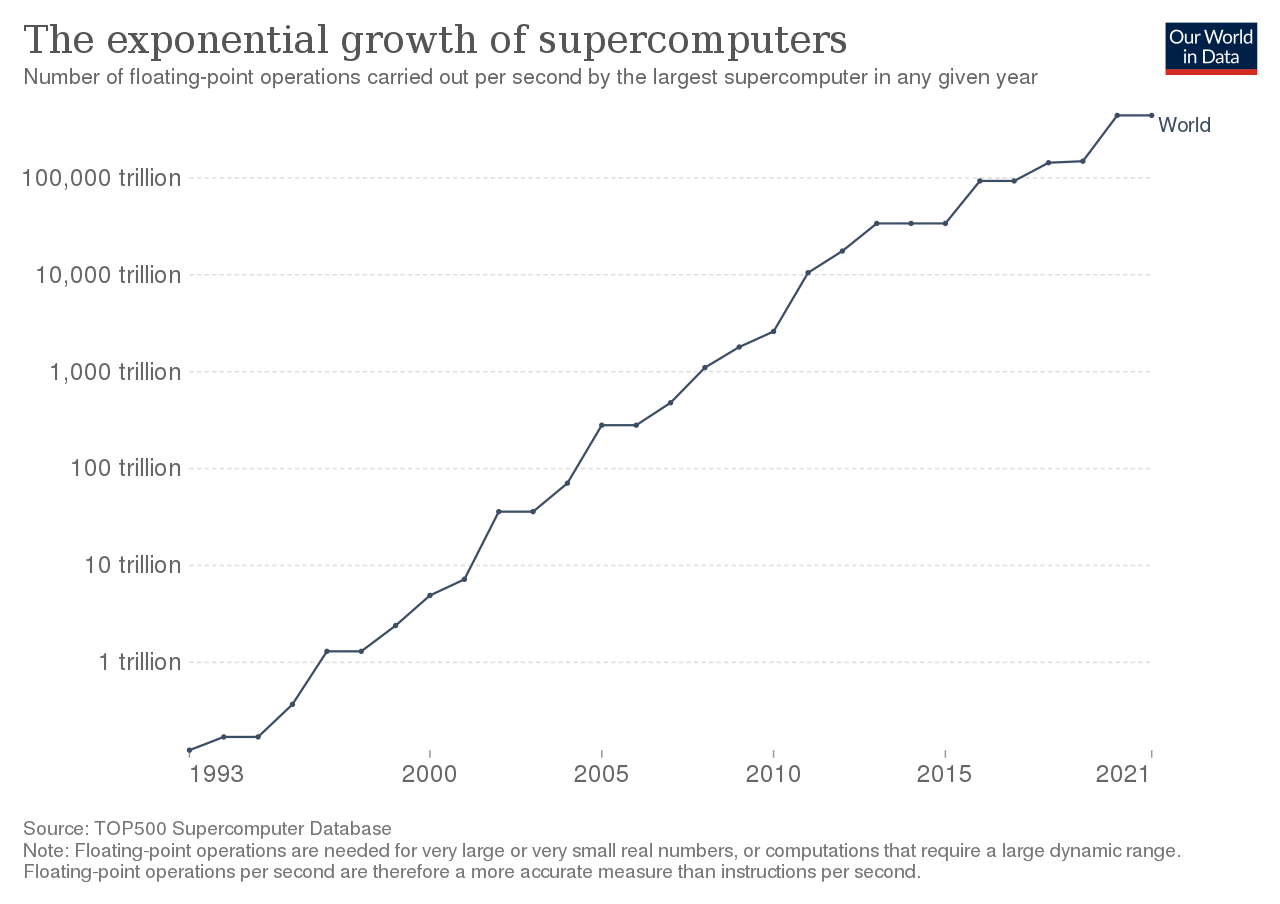
\includegraphics[width=0.7\textwidth]{Supercomputer-power-flops.png}
	\caption{Visualisation of supercomputer growth \cite{supercomputer-power-flops}}
	\label{fig:supercomputer-power-flops}
\end{figure}

This 60 year period of innovation and improvement in super-computing architectures, and processor technology has caused this technology to mature very quickly and is now used across the globe for a huge number of tasks each day. Stock markets, bank transfers, digital currencies, weather prediction and modelling, climate research are all run by HPC systems.

\phantomsection
\addcontentsline{toc}{subsubsection}{Scalability}
\subsubsection*{Scalability}
Common supercomputing architectures are now based around huge arrays of smaller computer systems, each using mostly off-the-shelf components \cite{sciences1989supercomputers}. This enables new supercomputing arrays to be set up very quickly and effectively, and at a considerably lower cost than a fully custom array would (though those systems do still exist) . It also makes them much more easier to upgrade and scale horizontally. Therefore, if a specific biological system requires more processing then it would be easy to simply add more nodes to the array and increase the capabilities of the system.

\phantomsection
\addcontentsline{toc}{subsubsection}{Ease of Setup and Maintenance}
\subsubsection*{Ease of Setup and Maintenance}
The environmental requirements of classical computers are not great. The major limitation (and cost) of HPC systems is the vast amounts of heat generated. The faster they are running, the more heat generated, requiring large amounts of cooling, either via HVAC or liquid cooling. Other than that, supercomputers can be set up anywhere there is enough space to fit it, and power for it to use.

Additionally, due to the modular nature of modern parallel systems, if a node fails, it can be easily hot-swapped out with a replacement.

\phantomsection
\addcontentsline{toc}{subsection}{Drawbacks of HPC}
\subsection*{Drawbacks of HPC}
A lot of current models for modelling biological systems are designed to model inert particles are not applicable to chemically inhomogeneous systems. The complexity of both the biological molecules and their interactions, due to the entropy of such systems. Calculating the energy levels and transfers between particles requires very detailed calculations, the number of which required scales exponentially as the number of molecules being simulated increases to fully model the system \cite{Quantum-assisted}.

Current Molecular Dynamics (MD) simulations can only simulate very small particles for very small periods of time. Using 32 CPUs to simulate a small protein, it is possible to simulate 100ns of the system in 24 hours of running the program. Therefore, to simulate that same protein with 162 ammino acids - approximately $3\times 10^{4}$ atoms - for $10\mu s$ would take 3200 CPU days \cite{MDsim}. 

Larger Molecules, for example, a ribosome, with $\approx 2.6\times 10^{6}$ atoms, being simulated for 20ns on 768 CPUs took $10^{6}$ CPU hours in 2006 \cite{Sanbonmatsu_2006}. Ribosomes produce one ammino acid every 100ms, and so to simulate the production with the same processing power, would take $10^{6}$ times longer, leading to almost 1.5 million years.

This is obviously impractical, and it is much more faster to just observe the actual system, partially due to the small time scales that biological molecules operate on and partially due to the complexity of the mathematics that underpins it.

Classical Processors are also, at their very core, linear. They can only process one instruction on one piece of data at a time. Whist running processors simultaneously can let one achieve parallel processing, there is a large amount of overhead required to coordinate each processor, which only increases as the number of processors increases.


\newpage
\FloatBarrier
\phantomsection
\addcontentsline{toc}{section}{Quantum Approach}
\section*{Quantum Approach}

\phantomsection
\addcontentsline{toc}{subsection}{Benefits of a Quantum Approach}
\subsection*{Benefits of a Quantum Approach}

\phantomsection
\addcontentsline{toc}{subsubsection}{Parallelisation}
\subsubsection*{Parallelisation}
A lot of the speed-ups from quantum computing relies on quantum parallelism, which arises from the ability for a quantum register (simply a place where qubits are stored) to exist in the superposition of base states. Applying a function/gate is performed on each of the components of the superposition, but due to the register being in a superposition, the function is only applied one time. The number of possible states is $2^{n}$, with n being the number of qubits in the register. Therefore, you can perform one operation on a quantum computer that would take an exponential number of operations on a classical computer.

For example, take the function (1), applied over a quantum register in an equally weighted superposition of the states 0 through 6, represented by $Q: \{0, 1, 2, 3, 4, 5, 6\}$:

\begin{align}
	f(x)          & = x^{2}+1                 \\
	\implies f(Q) & = \{1, 2, 5, 10, 26, 37\}
\end{align}

Although we have only performed the function once, every single component of the superposition has had the function applied to it. To perform the same operation on a classical computer, on the same data would require iterating over each element and performing the function on each number, 0 through 6, taking n iterations to complete, n being the number of elements performing the operation on.

However, as we increase the number of superposition states, we decrease the change that, upon measuring the quantum register and hence collapsing the superposition of states, that the desired value is measured. However, quantum algorithms can be designed to use properties of the output as a whole, not just a particular one.

This parallelism therefore can be utilised to speed up many problems and algorithms that, whilst possible on a classical system, would take a very large amount of time as the size of the problem increases.

\phantomsection
\addcontentsline{toc}{subsubsection}{Quantum Algorithms}
\subsubsection*{Quantum Algorithms}

\phantomsection
\addcontentsline{toc}{paragraph}{Defining Complexity}
\paragraph*{Defining Complexity}
\noindent
Algorithms and problems can be sorted into different complexities, which help one understand what problems can be efficiently solved, and the time and space their solutions take up. In \autoref{fig:Complexity Theory Classes}, we can see the relation between each class. P and NL are the two classes where problems can be solved in polynomial time, and a general rule of thumb is that any solution in these two classes can be efficiently solved and are tractable.

Quantum Algorithms, when properly designed, can exist outside of this P-complexity space, referred to as BQP (Bounded Quantum Polynomial). This contains any solution to a problem that can be solved in polynomial time on a quantum computer, but not a classical computer. \cite{doi:10.1137/S0097539796300921}

\begin{figure}
	\begin{figure}[H]
		\centering
		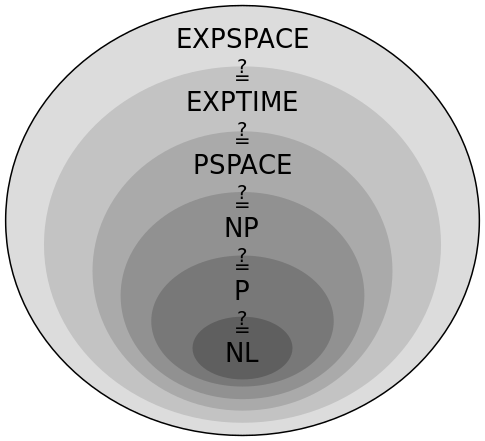
\includegraphics[width=0.4\textwidth]{Complexity_subsets_pspace.png}
		\caption{Complexity Theory Classes \cite{complexity}}
		\label{fig:Complexity Theory Classes}
	\end{figure}

\end{figure}

For example, integer factorisation. This is relied upon for many cryptography systems, such as RSA public-key encryption. RSA keys are composed of two semiprimes, numbers that are the product of two prime numbers. Whilst it has not yet been proven that the factorisation of prime integers is not a P-complexity space problem, the best publicly available algorithm currently has a time complexity of

\begin{align}
	O(\exp((\sqrt[3]{\frac{64}{9}}+o(1))(\ln{n})^{\frac{1}{3}}(\ln\ln{n})^{\frac{2}{3}}))
\end{align}
\noindent
for n number of bits. Whilst this is sub exponential, and therefore not in EXPTIME-complexity space, it does significantly exceed polynomial time. \cite{10.5555/270146}

\phantomsection
\addcontentsline{toc}{paragraph}{Shor's Algorithm}
\paragraph*{Shor's Algorithm}
\noindent
There is however, an algorithm devised by Peter Shor, which, using a quantum computer, can factorise large prime integers in polynomial time \cite{365700}.

\begin{align}
	O((\log{n})^{2}(\log\log{n}))
\end{align}

\noindent
This algorithm was first implemented in 2001, using a 7 qubit NMR quantum computer \cite{Vandersypen_2001}.
This is just one example of a problem that can be significantly sped up by designing quantum algorithms. If this algorithm can be scaled up, it provides a significant threat to cryptography.

\phantomsection
\addcontentsline{toc}{paragraph}{Differential Equation solvers}
\paragraph*{Differential Equation solvers}
\noindent
Many, if not all mathematical and scientific models are underpinned by differential equations. They are used to describe how functions interact with their derivative and change in relation to other variables. Some common differential equations include:

\begin{align}
	\frac{d^{2}u}{du^{2}}+\omega^{2} u                                                                                                    & = 0 &  & \text{Describing a harmonic oscillator}                 \\[0.5em]
	L\frac{d^{2}}{du^{2}}+g\sin{u}                                                                                                        & = 0 &  & \text{Describing the motion of a pendulum, length L}    \\[0.5em]
	\nabla^{2}f(x, y, z) = \frac{\partial^{2}f}{\partial x^{2}}+\frac{\partial^{2}f}{\partial y^{2}}+\frac{\partial^{2}f}{\partial z^{2}} & = 0 &  & \text{3-dimensional Laplace equation \cite{laplace_eq}}
\end{align}

\noindent
The speed with which we can either, find a solution to a differential equation (that is, find functions that represent each of the variables involved), or find a numeric solution to the differential equation, therefore plays a large role in the speed that we can model biological systems.

For both linear (the system only contains linear equations of u and it's derivatives), and non-linear (system contains non-linear functions of u and it's derivatives) differential equations, there exists quantum algorithms for solving both. Classical algorithms for solving differential equations typically grow exponentially with the number of variables involved. However, using quantum algorithms this can be reduced to poly-logarithmic time or better \cite{10.48550/arxiv.2011.06571,10.48550/arxiv.0812.4423}, and for linear differential equations, even to quadratic time ($O(n^{2})$) \cite{Berry_2014}.


\phantomsection
\addcontentsline{toc}{paragraph}{Fast Fourier Transform}
\paragraph*{Fast Fourier Transform}
\noindent
The Fourier Transform is a mathematical transform that decomposes a function into it's frequency components. For example, splitting a musical waveform into the intensity of the individual pitches and harmonics. However, it has many uses, including solving partial differential equations.

The Fast Fourier Transform (FFT) was (re)discovered by James Cooley and John Turkey in 1965, thought the be an original discovery at the time, but it was later found that Carl Gauss had already devised it over 160 years earlier \cite{cooley_tukey_1965}. This algorithm was pivotal in a giant number of fields, reducing the time complexity to perform a Fourier transform from $O(n^{2})$ to $O(n\log{n})$. In \autoref{fig:FFTcompare} it is clear that the FFT scales much more slowly than traditional methods, as the dimensions of the input matrix increases.

\begin{figure}[H]
	\centering
	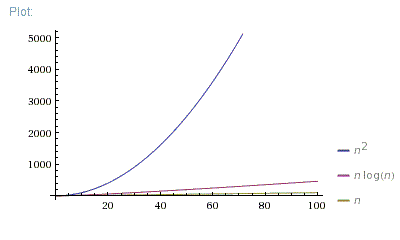
\includegraphics[width=0.58\textwidth]{PB0M1.png}
	\caption{$O(n^{2})$ vs $O(n\log{n})$ vs $O(n)$}
	\label{fig:FFTcompare}
\end{figure}

\phantomsection
\addcontentsline{toc}{paragraph}{Quantum Fast Fourier Transform}
\paragraph*{Quantum Fast Fourier Transform}
\noindent
A quantum algorithm also exists to perform an FFT on a quantum system, and when implemented properly can scale at $O(n)$ \cite{asaka_sakai_yahagi_2020, Quantum-assisted}. See \autoref{fig:FFTcompare} \\ \\

\noindent
The exponential speed up - along with the quantum parallelism discussed earlier - provided by quantum algorithms can vastly increase the speed and efficiency that we can simulate biological systems with, especially as the number of variables and particles simulated grows.

\phantomsection
\addcontentsline{toc}{subsection}{Drawbacks of a Quantum Approach}
\subsection*{Drawbacks of a Quantum Approach}
Whilst this paints a rather favourable picture for quantum computing matching and superseding HPC in the field of computational biology, there exists a number of significant drawbacks.

\phantomsection
\addcontentsline{toc}{subsubsection}{Quantum Effects}
\subsubsection*{Quantum Effects}
Whilst quantum computing as a concept has been around for over 4 decades, the actual capabilities to construct and maintain quantum computers have only come to fruition recently, with huge corporations and small start-ups producing systems using various designs. However, regardless of the design philosophy used in a quantum computer, it is still very difficult to maintain the entanglement of many qubits at once, and this only becomes more difficult as the number of qubits increases. Entanglement of qubits is critical to many quantum gates functioning. The greater the number of entanglement qubits, the greater the number of states that computer can represent and be in a superposition of.

Additionally, qubits need to be entangled with each other, but not entangled with anything else; They must be designed very carefully not to entangle with any other physical system and therefore become decoherent.

Qubits must also be shielded from any kind of interferences, such as radiation or other particles. Some decoherence and noise is inevitable in any quantum system, however our techniques to manage these factors are relatively immature and limit the ability to scale quantum systems. For example, we can create a "logical" qubit that is composed of many entangled qubits to represent one noise-free qubit. However, it is estimated that 100 to 1000 physical qubits are required to create one logical qubit, which brings us back to the issue of maintaining coherence between qubits.

Qubits are not just isolated units. Quantum computers need to be able to control and measure each qubit's state, requiring large amounts of circuitry, and this increases linearly as the number of qubits increases. If using a logical qubit system, this would exacerbate this issue even more.

Decoherence limits the amount of time we can run quantum computers for before the error rate becomes too high to take any meaningful reading. If we wanted to simulate a biological system that acts over a couple of days, then we would currently have significant challenge maintaining coherence during that timescale.

\phantomsection
\addcontentsline{toc}{subsubsection}{Cost}
\subsubsection*{Cost}
Whilst the construction of quantum computers is not cheap - Dwave's 2000 qubit quantum computer has a price tag of \$15 million, it is the cooling and power requirements of quantum systems that really increases the cost.

\phantomsection
\addcontentsline{toc}{paragraph}{Cooling}
\paragraph*{Cooling}
\noindent
Qubits must be cooled to temperatures just above absolute zero in order to reduce the effect of heat radiation, and also to stabilise the qubit. In quantum systems that use superconducting magnets, cooling is also required for those magnets to superconduct. Cooling lasers are used to freeze qubits and held, whist being manipulated and measured using other qubits.
The costs are due to the high energy requirements of these lasers, and cost of supercooled fluids like Helium.

\phantomsection
\addcontentsline{toc}{subsubsection}{Classical Processing}
\subsubsection*{Classical Processing}
Whilst many quantum algorithms can provide exponential speed-ups over classical equivalents, many of these algorithms require additionally processing, either via another quantum algorithm or via processing on a classical system. This is due to qubits being superposed, and the need for individual state's probabilities needing to be measured. This post-processing can actually nullify the benefits one gains when running quantum algorithms, and can even make some algorithms scale worse than their classical counterparts. 

Additionally, the scaling of a quantum algorithm does not show the whole picture. Whilst in theory a quantum algorithm may scale more efficiently that a classical equivalent, it does not mean that the specific implementation of a quantum computer can complete the computation quicker than a classical computer.


\newpage
\FloatBarrier
\phantomsection
\addcontentsline{toc}{section}{Potential Solutions}
\section*{Potential Solutions}

\phantomsection
\addcontentsline{toc}{subsection}{Encode the entire system in superposition}
\subsection*{Encode the entire system in superposition}
This would use quantum parallelism to mimic the way that current classical algorithms work. That single classical computation could be carried out using an exponentially smaller amount of memory, but in turn, only provide a very small portion of data. This is therefore only suitable for simulations where the desired result is some global average that can be extracted from the probability of each state in memory. It also would require the whole computation to maintain coherence for the entire computation, and therefore is not likely to be suitable for modelling large biological systems where intricate detail is required.

\phantomsection
\addcontentsline{toc}{subsection}{Perform multiple computations in superposition}
\subsection*{Perform multiple computations in superposition}
The system would be encoded the same way a classical simulation would be, resulting in no saved memory, but the quantum superposition still allows one to perform several computations in parallel. A single simulation could processes different initial conditions, each encoded separately simultaneously. The most favourable outcomes could then be selected using destructive interference of less favourable outcomes. 
Multiple simultaneous computations could also be used to calculate the entropy of each molecule in the system, a variable that is often poorly estimated in classical models due to its high complexity, which would vastly increase the accuracy of simulations.

\phantomsection
\addcontentsline{toc}{subsection}{Quantum Subroutines}
\subsection*{Quantum Subroutines}
A hybrid approach could be used, in which computations that are inefficient on a HPC are ran on a quantum computer. This means that quantum coherence only has to be maintained for the length of the timestep of the simulation, and so may be feasible sooner. The running time of the simulation would be decreased by the time factor that each time-step is decreased by.   

\newpage
\FloatBarrier
\phantomsection
\addcontentsline{toc}{section}{Evaluation}
\section*{Evaluation}

High Performance Computing is going nowhere anytime soon, and will continue being the backbone of our computational needs for the forseeable future. It is low cost, highly scalable and can be set up in most environments. To be able to utilise the abilities that computational biology would provide us in the near future, HPC is the most viable option, and as processor and GPU technology improves, so will the performance of HPC. \\

\noindent
Whilst quantum computing can provide us with incredible benefits and speed-up over classical 
computing, the technology still is not mature enough to provide much usefulness. There are many problems, such as the issue of coherence and scalability, that will have to be solved before quantum computing will become competitive. Additionally, even if we do eventually develop large scale quantum systems, I do not believe that they will fully replace our HPC systems that are already deployed. Some classical algorithms just cannot be sped up using quantum computers and so the additionally costs and complexity that comes with running said algorithm on a quantum system is not worth it. 

After all, quantum computers are a completely different type of computer, not just an evolution of our current technology. There are so many problems that can be solved on a quantum computer that are just inconceivable on a classical computer, and so it is not injust to look at it in an opposite way.  \\ 

\noindent
When modelling biological systems, there are no quick and easy solutions when simulating large, complex systems with many variables. However, quantum computers have very special capabilities and features that, when properly developed and mature, could make a significant difference to our prediction and modelling of biological systems. Most important of those features is the ability for a quantum system to process multiple versions of simulations simultaneously, that would allow the finding of the minimum free energy. Modern MD simulations now include repeat simulations, in which a number of initial confirmations are investigated in parallel to check the robustness of any conclusions against thermal noise \cite{Quantum-assisted}. The potentially huge parallelisation provided by quantum computers could take this to the extreme, modelling hundreds of different starting conditions simultaneously. \\

\noindent
I therefore believe that Quantum Computers will only partially replace high performance classical computing in the field of computational biology. Whilst quantum computers can theoretically perform algorithms and functions critical to biological modelling, such as the Fast Fourier Transform and solving differential equations with a much greater efficiency than classical computers, there are many issues that prevent quantum computers fully replacing classical systems:

\begin{enumerate}
	\item Maintaining Coherence - Quantum systems cannot maintain coherence for the long  timescales that some modelling may require.
	\item Cooling - To ensure that the amount of noise in the quantum system is as low as possible, quantum systems must be cooled to as low a temperature as possible. This requires large amounts of extra infrastructure and considerations when designing large scale quantum systems.
	\item Nature of Superposition - Whilst some algorithms can exploit the features of superposed qubits, as the number of states contained within the superposition increases, it becomes more and more difficult to extract the desired value without having to do extra processing on top, which will scale with the number of superposed states in itself, potentially nullifying the benefits gained from quantum parallelism. 
\end{enumerate}


I think the most probable outcome is that we see hybrid quantum-classical supercomputers, where computations that can be made more efficient (that is, scale less as the number of inputs increase) by using a quantum approach are offloaded to quantum systems, where as computations that would provide no benefit, or even be slower on a quantum computer are kept on a classical machine. We have already seen this demonstrated by various companies that provide access to quantum computers over the cloud. Users interface with a classical computer to write the code to be executed on the quantum computer, and the classical system then measures the quantum state, providing an output to the user.  

\bibliographystyle{ieeetr}
\phantomsection
\newpage
\bibliography{bibliography.bib}
\end{document}
